
\documentclass[12pt,a4paper,titlepage]{report}
%\documentclass[a4paper,12pt]{article}
\usepackage[utf8x]{inputenc}
\usepackage{amsfonts}
\usepackage{fancyhdr}
\usepackage{titlesec}
\usepackage{tocloft}
\usepackage{listings}
\usepackage[T1]{fontenc}
\usepackage{ascii}
\usepackage{graphicx}
\usepackage{pifont}
\usepackage{float}
\usepackage{sidecap}
\usepackage{wrapfig}
\usepackage{titletoc}
\usepackage{tocloft}
\usepackage[nottoc]{tocbibind}
\usepackage{afterpage}
\usepackage[right=25mm,left=35mm,top=25mm,bottom=25mm]{geometry}
\usepackage[parfill]{parskip}
\usepackage{comment} 
%\usepackage[a4paper]{geometry}
\usepackage[numbers]{natbib}
\usepackage{balance}
\usepackage[table]{xcolor}
\usepackage{color}
\usepackage{amsmath}
\usepackage[inference,shorthand]{semantic}
\usepackage{bm}
\usepackage{booktabs}
\usepackage{array}
\usepackage{tikz}
\usepackage[]{caption}
\usetikzlibrary{mindmap,trees}

\newcommand{\head}[1]{\textnormal{\textbf{#1}}}
\newcommand{\normal}[1]{\multicolumn{1}{l}{#1}}
\newcommand{\hilight}[1]{\colorbox{yellow}{#1}}	
\addtocontents{toc}{\protect\renewcommand{\protect\cftchapleader}{\bfseries\protect\cftdotfill{\protect\cftdotsep}}}
\newenvironment{cmd}{\fontfamily{ascii}\footnotesize\selectfont}{}
\setcounter{secnumdepth}{3}
\setcounter{tocdepth}{3}

\titleformat{\chapter}[hang]{\huge}{\thechapter}{1em}{}
\titlespacing{\chapter}{0pt}{0pt}{1cm}

\pagestyle{fancy}
\fancyhead{}
\fancyfoot{}

\setlength{\headheight}{15pt}
\addtolength{\textwidth}{2cm}
\addtolength{\hoffset}{-1cm}

\fancyfoot[C]{\thepage}
\renewcommand{\headrulewidth}{0pt} 
\renewcommand{\chaptername}{}

\usetikzlibrary{shadows,arrows,positioning}



\begin{document}



%%%%%%%%%
%%%%%%%%%%%%%%%%%%%% Title page %%%%%%%%%%%%%
%%%%%%%%%

\begin{titlepage}
\vspace*{\fill} % Vertical Align
\begin{center}

% Uni stuff


%	LOGO SECTION
%----------------------------------------------------------------------------------------


\includegraphics[width=0.5\textwidth]{logo.jpg}\\[1.4cm] 

%----------------------------------------------------------------------------------------



% Title
\textbf{\LARGE Platform for Microrobot Navigation} \\ [1.5cm]


% Author and date
{\LARGE Nafiseh Vahabi} \\ [1.3cm]


% Report title
{\LARGE \lq{}\lq{}A thesis submitted in partial fulfilment of the } \\ [0.3cm]
{\LARGE requirements for the degree of MRes in }\\ [0.3cm]
{\LARGE  Medical Robotics and Image Guided Intervention}\\ [0.3cm]
{\LARGE  and for the Diploma of Imperial College\rq{}\rq{}}\\ [1.3cm]


{\LARGE Imperial College London} \\ [0.8cm]

{\LARGE \today} \\ [1.5cm]

% Examiner details
{\LARGE Project supervisors: Dr. Henry lp, Dr. Vincenzo Curto} \\ [0.3cm]
{\LARGE and  Professor Guang-Zhong Yang} \\ [1cm]




\end{center}
\vspace*{\fill}
\end{titlepage}

%%%%%%%%%
%%%%%%%%%%%%%%%%%%%%END Title page %%%%%%%%%%%%%
%%%%%%%%%

\pagenumbering{roman}

%\section{Acknowledgements}
\addcontentsline{toc}{chapter}{\numberline{}Acknowledgements}
%\pagenumbering{roman}
\setcounter{page}{1}
\thispagestyle{plain}
\chapter*{Acknowledgements}

I would like to thasnks to 
\pagebreak


\renewcommand{\cftsecleader}{\cftdotfill{\cftdotsep}}
\tableofcontents
%\setcounter{secnumdepth}{2}
%\setcounter{page}{1}

\pagebreak



%\addcontentsline{toc}{chapter}{\numberline{}List of Figures}
\setcounter{page}{3}
%\thispagestyle{plain}
\listoffigures
%\chapter*{List of Figures}
\pagebreak



%\addcontentsline{toc}{chapter}{\numberline{}List of Tables}
\setcounter{page}{4}
%\thispagestyle{plain}
\listoftables
%\chapter*{List of Tables}
\pagebreak




%------------------------------------------- Abstract -------------------------------------

\begin{abstract}
\addcontentsline{toc}{chapter}{\numberline{}Abstract}
%abstract

Structures and functions of microorganisms were made them suitable reference to design
 microrobots. Flagellar propulsion of microorganism such as E.coli is used as an efficient approach for 
modelling micro swimmers locomotion method in low Reynolds number regime. Microrobots were 
demonstrated precise and controllable movements under low strength magnetic field. A system with 
a size of bacteria, capable to swim in viscous fluid in a controllable manner was satisfied basic principles
 for performing delicate tasks such as targeted drug delivery in medical application. Furthermore 
microrobots were advantaged from fabrications technology to make them biocompatible. We review 
a range of bio mimetic microrobots and their fabrication methods and reproduce helical micro 
swimmers by analysing their mathematical propulsion methods. The definitive microrobots designs 
were simulated and printed by Nanoscribe technology. Finally,  








%\pagenumbering{roman}
\setcounter{page}{5}
\thispagestyle{plain}

\end{abstract}

%-------------------------------------------END Abstract -------------------------------------

\pagenumbering{arabic}

%%%%%%%%%
%%%%%%%%%%%%%%%%%%%% Introduction %%%%%%%%%%%%%
%%%%%%%%%
\chapter{Introduction}


The potential use of microrobots in medical applications such as minimally invasive surgery 
has attracted scientists to work on designing microrobots ~\citep{edd2003biomimetic}. research into swimming 
microrobots showed two primary difficulties are the power source and finding suitable locomotion methods, as
 there are many cells, proteins and fibres in biofluids that prevent the motion of the microrobots~\citep{peyer2013bio}. 

Artificial bacteria flagella is most popular microrobots were inspired by nature~\citep{qiu2014noncytotoxic}. 
They have helical shape, are composed of magnetic material and are capable to mimick three dimentional 
motion of the bacteria in a high viscous fluid.

Magnetically actuated helical micromachines can be used
 in a variety of biomedical applications such as cell characterisation, targeted drug delivery and in vivo 
diagnosis ~\citep{peyer2013magnetic}. However, the issue of biocompatibility and the materrial 
used to make a microrobot needs to be considered carefully for in vivo application\citep{qiu2014noncytotoxic}. 
Section \ref{fabrication} presents a prief histery of fabrication techniques and section \ref{microFabric} describes
 the fabrication method is applyed in this study.     
In addition, the extremely small size of the microrobots and the
complex biofluid environment make the design aspect very challenging. 


\paragraph{}
The design of microrobots depends on their application and the desired task. An overview of the different
 microrobot designs, their structures and fabrication methods are discussed in the chapter 2, literature review, .

\paragraph{}
For the purpose of this project different proposed structures of microrobots were studied
 and analysed. This will enable helical microswimmers to be reproduced. Once reproduced, the aim of this project will be to compare
 the efficiency, power, motion velocity and cost-efficiency of various microrobot designs for mass production
 of the microswimmers. The fabrication of microswimmers will be by Nanoscribe facility using 3D laser
 lithography. After the microrobots are produced their characteristic will be analysed
 under the scanning electron microscope in order to identify further improvements in microrobot design. 


\begin{figure}
\centering
\pagestyle{empty}
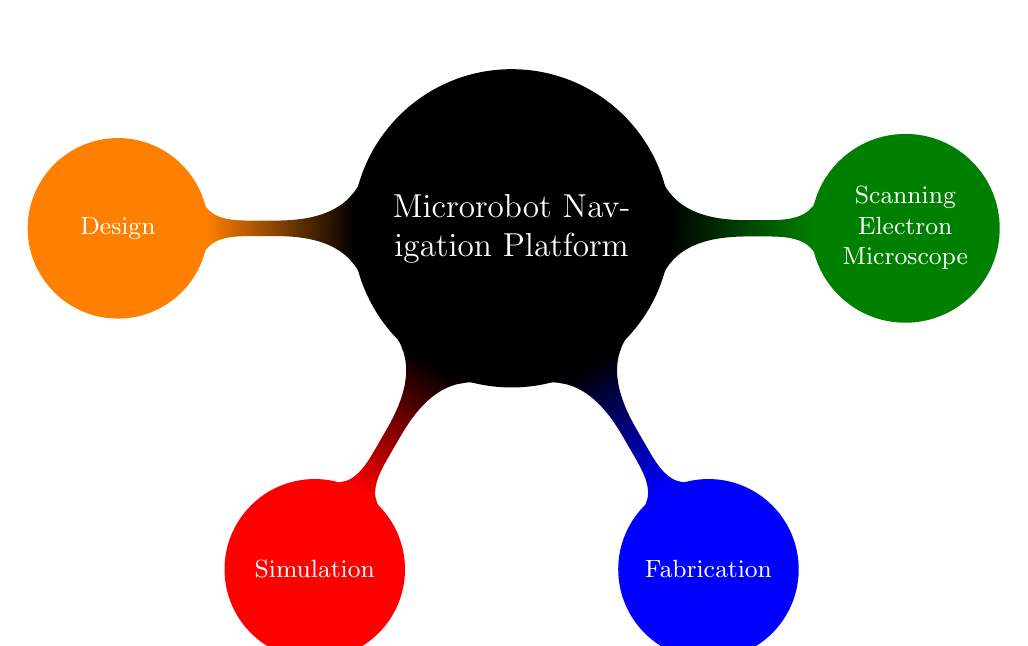
\begin{tikzpicture}
  \path[mindmap,concept color=black,text=white]
    node[concept] {Microrobot Navigation Platform}
    [clockwise from=0]
    child[concept color=green!50!black] {
      node[concept] {Scanning Electron Microscope }
      [clockwise from=90]
      %child { node[concept] {algorithms} }
      %child { node[concept] {data structures} }
      %child { node[concept] {pro\-gramming languages} }
      %child { node[concept] {software engineer\-ing} }
    }  
    child[concept color=blue] {
      node[concept] {Fabrication}
      [clockwise from=-30]
      %child { node[concept] {databases} }
      %child { node[concept] {WWW} }
    }
    child[concept color=red] { node[concept] {Simulation} }
    child[concept color=orange] { node[concept] {Design} };
\end{tikzpicture}

\caption{Project overwiew. This diagram shows different aspects of the project.  }						   
\label{Overview}										   
\end{figure}


\section{Problem}

\section{Previous work}


%%%%%%%%%
%%%%%%%%%%%%%%%%%%%% literature review %%%%%%%%%%%%%
%%%%%%%%%

\chapter{Literature review}
 


\section{Bioinspired microrobots}

One of the most challenging aspects of designing a robot on a very small scale such 
as a nanorobot is simplicity. The reason is, integration will become unfeasible on that
 scale if the design is complex. Hence the development of the nanorobot or even microrobot
 should be based on the essential functionality, avoiding any unnecessary components~\citep{gao2013bioinspired}.
By learning from nature and mimicking the structure of live organisms, the successful  
scientific applications were created~\citep{qiunanohelices}. In the following section a
 few examples of microrobots that were imitated from nature will describe. 
 



\paragraph{Reynolds number}

To understand how micro organisms swim in a fluidic environment, it is essential to study their propulsion 
mechanism. In the fluidic regime the Reynold number (Re) has a substantial effect on a microdevice
locomotion~\citep{peyer2013magnetic}. The Reynolds number describes the ratio of the inertial forces versus viscous 
forces according the following formula;

\begin{equation}
  Re = \cfrac{UL\rho}{\mu}
\label{eq:4}
\end{equation}
 
Where $ U$ is velocity, $L$ is characteristic length, $\rho$ is the density and $\mu$ is viscosity of the fluid.






\subsection{Flagella style microrobots}

Helical flagella and cilia are two well-known microswimers in nature that have had their functionality employed 
for motion generation in artificial microrobots  (Figure~\ref{cilia}) ~\citep{gao2013bioinspired}. 



\begin{figure}
  \centering
    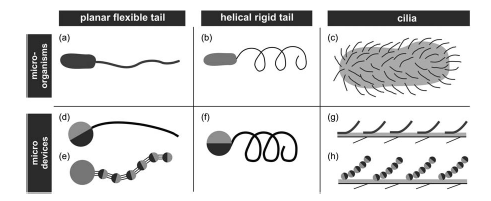
\includegraphics[width=0.9\textwidth]{cilia}
  \caption{The illustration of both flagellum and cilia shapes and microdevices mimicked the flagellum and cilia 
structures.~\citep{peyer2013bio}.}
  \label{cilia}
\end{figure}

In 2007, Bell ~\citep{gao2013bioinspired} presented the first artificial bacteria flagellum microrobots and then
 Zhang characterised them in 2009 ~\citep{gao2013bioinspired}. This microrobot was formed of two 
components; a rigid helical tail and a soft magnetic metal head. The head diameter 
was $2.8 \mu  m$ and its length was $30-100 \mu m$. Since then, other scientists proposed a slightly different design 
structure, that all have the rigid helical tail structure. However, in some cases the magnetic
 materials is used in the device tail rather than the head ~\citep{gao2013bioinspired}. 
 
\paragraph{}

%\begin{figure}
%  \centering
\begin{wrapfigure}{r}{0.5\textwidth}
  \begin{center}
    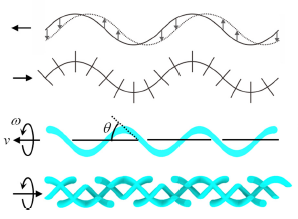
\includegraphics[width=0.5\textwidth]{10}
  \caption{ The structure of the smooth flagellum and a mastigonemes flagellum.~\citep{gao2013bioinspired}.}
  \label{10}
\end{center}
\end{wrapfigure}
%\end{figure}

The helical rotation of flagella and the travelling wave beat of cilia are two non-reciprocal propulsion
 mechanisms in microorganisms. Mimicking a rotating flagellum at low Reynolds number to generate an 
adequate torque to overpower the high viscous drag requires two main elements; a rotary motor and a
 power source ~\citep{qiunanohelices}. 
An electromagnetic rotary motor can be used in designing a helical flagella style microrobot that 
requires a considerable current. However piezoelectric rotary motors are an alternative option 
that are appropriate for miniaturisation but necessitate high input voltage.  Hence, designing a microrobot with a 
combination of an onboard power source and a motor is a challenging task ~\citep{qiunanohelices}.

Another design of microswimmers was inspired by the function of magtigonemes in nature ~\citep{tottori2013artificial}.
 A smooth flagellum moves against the direction of the propagation of the flagella wave. However, 
the flagellum covered by magtigoneme propels in the same direction as the flagellum wave (Figure~\ref{10}). Mimicking 
the structure of flagellum and using 3D lithography and electron beam evaporation formed the fabrication 
method in these microswimmers.
The anisotropic viscous drag on the flagella is an important fact for locomotion in low Reynolds number fluid. 
Flagella movement in the opposite direction of the flagella wave is because the 
viscous drag coefficient perpendicular to the flagella is greater than the viscous drag coefficient parallel to 
the flagella~\citep{tottori2013artificial}. 

 The rotating field, i.e. rotational frequency, field strength and angles that 
defined the rotational axis can be controlled by the current in the external coil. The helical microrobots rotate 
synchronously with the rotation of the magnetic field and move forward and backward accordingly ~\citep{tottori2013artificial}. 
The displacement of the microswimmer along the rotational axis can be measured and the result 
used to calculate the average velocity of the swimmers. There is a linear relationship between an input 
field frequency and swimming speed. According to their result ~\citep{tottori2013artificial}, a propulsive force generated by 
the mastigoneme is in opposite direction of the force generated by the main helical filament. 
However, this velocity is only valid if the external force is zero. The proposed 
design ~\citep{tottori2013artificial} is rigid and an external stimulus may be used to regulate the swimming
 speed and direction if the swimmer can fold and unfold their structure. 


There are three common shapes of microrobots 
based on the rotary action; a helix, a screw and a twisted ribbon shape around its
 axis (Figure~\ref{HelixShapes}). For the purpose of drilling into solid matter such as biological tissue the screw and helix 
design would be more appropriate. The rotational motion of helical micro
 swimmers is one of the most effective propulsion methods in the low Reynolds number scenarios 
because it leads to translational motion. Microrobots with the microspheres structure perform similarly 
to the helical swimmers and are capable of swimming in the flowing liquid within the microfluidic channel~\citep{kim2013fabrication}. 


%\begin{figure}
%\begin{SCfigure}
  %\centering
\begin{wrapfigure}{r}{0.5\textwidth}
  \begin{center}
    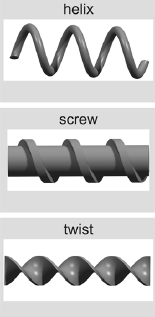
\includegraphics[width=0.4\textwidth]{HelixShapes}
  \caption{Three design of helical microswimmers.~\citep{peyer2013magnetic}.}
  \label{HelixShapes}
  \end{center}
\end{wrapfigure}
%\end{SCfigure}
%\end{figure}



There are two main factors that affect the movements of the microrobot in the external magnetic
 field; \hilight{low coercivity and high saturation} magnetization. Also, the motion of the microrobot is related to 
its size given the same magnetic field strength and as such, by increasing the size of the microrobot with the inflexible magnetic material
 volume, the velocity will decrease ~\citep{kim2013fabrication}. 
The surface friction and the drag forces are two resistive forces that impede the microrobot\rq{}s 
motion. Hence, the input magnetic force must be sufficient to overcome these forces for microrobot 
manipulation. Furthermore, the weight of the microrobot requires gravity compensation in the z-direction by 
the magnetic field. The navigation methodology should compensate for gravity to avoid sinking and enable velocity to be 
controlled wirelessly. \citeauthor{mahoney2011velocity} described an algorithm for helical microswimmers velocity 
control plus gravity compensation. In the proposed model the correct pitch angel and 
rotation speed is calculated to achieve the commanded velocity (Figure~\ref{11}).


\begin{figure}
  \centering
    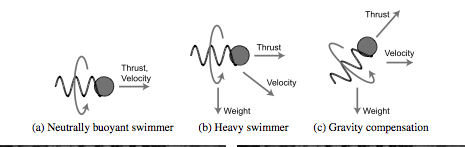
\includegraphics[width=0.9\textwidth]{11}
  \caption{The effect of the gravity on the microrobot motion direction and gravity compensation~\citep{mahoney2011velocity}.}
  \label{11}
\end{figure}


The mathematic model below describes the microrobot translational movement;

\begin{equation}
  \overrightarrow{F_m }+ \overrightarrow{F_r} - \overrightarrow{F_g} = M(\overrightarrow{dv}/dt)
\label{eq:4}
\end{equation}

Where $F_m$, $F_r$ and $F_g$ are a magnetic force, overall resistive force and gravitational force respectively. 
$M$ is a mass and $v$ is a translational velocity of the microrobot~\citep{kim2013fabrication}. 

A magnetic field can be used for controlling teams of microrobots as well as a single 
one. \citeauthor{kim2013fabrication} proposed a method that used a combination of two magnetic materials to 
attain on/off magnetization of each microrobot. The overall control of the group of microrobots 
was achieved by managing the magnetization state of each microrobot. In addition, a second technique has been 
developed for three-dimensional motion of the team of microrobots in a fluidic environment. In
 the latter method, each microrobot is designed in such a way that it uniquely responds to the 
input magnetic field. Therefore, several microrobots can provide feedback position control in 
3D system~\citep{kim2013fabrication}.
An untethered spherical magnetic micromanipulator creates a locally induced rotational fluid flow gradient. 
The created rotational flow propels micro-objects in the flow area. A team of microrobots could perform
 a complex task in micro-transport and micro-assembly~\citep{kim2013fabrication}.

In another study ~\citep{tottori2012magnetic}, a helical microrobot was designed to swim in a low Reynolds number. 
Two designs are selected to run the experiment;  the first one is a bare helical structure and the second one is the
 helical shape with the microholder attached at the end. Both designs will generate the corkscrew
 motion in a fluid environment when the magnetic filed is about few mili Tesla. The second 
design (device with the microholder) is capable of transporting a microobject accurately to the 
target ~\citep{tottori2012magnetic}.\hilight{size and weight of the object}


%\begin{figure}
  %\centering
\begin{wrapfigure}{r}{0.5\textwidth}
  \begin{center}
    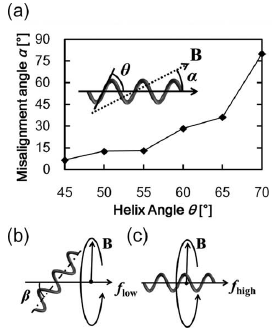
\includegraphics[width=0.5\textwidth]{7}
  \caption{(a) The misalignment of helical angle$\alpha$ with differnt helix angle (b) the oscillation behaviour
of the microswimmer with the high and low frequencies ~\citep{tottori2012magnetic}.}
  \label{ref7}
\end{center}
\end{wrapfigure}
%\end{figure}


In ~\citeauthor{tottori2012magnetic}\rq{}s study eight designs of microrobots were proposed and tested. 
The uniform static magnetic field was used to explore the magnetic shape anisotropy and the 
magnetic actuation was monitored in the rotating magnetic field. In the static magnetic field the 
set of microrobots had helical angles $\theta$ ranging from ${45^{\circ}}$ to ${70^{\circ}}$ when suspended in the deionised water. 

This showed (Figure~\ref{ref7}) that a smaller helix angle $\theta$ results in a less misalignment 
angle $\alpha$ because microrobots longest axes will be aligned to the direction of the external magnetic field. 
However in helical microrobot with larger helix angles ($\theta$), the magnetization direction would change to 
the radial axes of the helix  ~\citep{tottori2012magnetic}.
In the rotating magnetic field, the micro helical swimmer exhibits different behaviours depending on 
the strength of the applied frequency in the fixed magnetic field. At low frequencies the micro helix oscillated 
around the helical axes, however the oscillating behaviour changed to the 
corkscrew motion after increasing the applied frequency in the magnetic field. This is similar to characteristics of 
microrobots with an incorporated
 microholder~\citep{tottori2012magnetic}.

The velocity of helical micro swimmers depends on their size and shape. A linear relationship was 
observed between the input frequencies and swimming velocity of the micro swimmers. The outcome of 
the comparison between three microhelixs with the same helix angles showed that the microhelix with the
 greatest diameter has the highest speed, in accordance with the following formula;

\begin{equation}
  U = {\cfrac{(C_n - C_1) \sin \theta \cos \theta}{2(C_n \sin^2 \theta + C_1 \cos^2 \theta)}} \big( d \varpi \big)
\end{equation} 

Where $C_n$ is a drag coefficient perpendicular to the filament and $C_1$ is a drag coefficient
 parallel to the filament. $ \varpi$ is the rotational frequency and $d$ is the rotational diameter of 
the helix ~\citep{tottori2012magnetic}.  



\paragraph{}
The important role of helix angle in the magnetization structure of helical micro swimmers 
was confirmed by \citeauthor{peyer2013bacteria} \citep{peyer2013bacteria}, who used direct laser writing (DLW) as a fabrication method but 
applied (DLW) on a magnetic polymer composite (MPC). The MPC are non-cytotoxic and showed 
super paramagnetic characteristic because magnetic material was already included in the polymer. 

The relationship between the torque $T$, the drag force $F$, the object\rq{}s velocity $\nu$ and rotational 
speed $\omega$ is linear and modelled by $6\times6$ resistant matrix as below;



\[
\begin{bmatrix} F\\ 
T \end{bmatrix}  =\begin{bmatrix} A & B \\ 
C & D \end{bmatrix}  \begin{bmatrix} \nu
 \\ \omega
\end{bmatrix}
\]




Where $A$, $B$ and $D$ are matrices 3x3 and only depend on the object\rq{}s geometry and fluid velocity.
In the study performed by \citeauthor{purcell1997efficiency} \citep{purcell1997efficiency} has been proved 
matrices $B$ and $C$ are equal ($B = C$) for a typical flagellum. 
There are few methods in use to model the resistance matrices and low Reynolds flow such as the 
method of regularized stokeslets, the boundary element method and the method of fundamental solution
. In designing a microrobot the main parameters required to concentrate on are the helicity angle $\psi$, 
the helix radius $R$, the pitch $p$ and the filament radius $r$ as illustrated in Figure~\ref{ref8} part (c). 
The details of above methods will discuss in section \ref{maths} (Mathematical model).

\begin{figure}
  \centering
    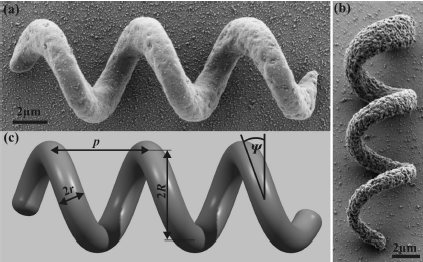
\includegraphics[width=0.7\textwidth]{8}
  \caption{ The prototype of microhelical device. (a) Scanning electron microscopic image of the micro polymer composite
with the 2 vol.\% nanoparticle fill factor and (b) 4 vol.\% of nanoparticle fill factor. (c) The CAD model
shows all the parameters required for the microhelical design ~\citep{peyer2013bacteria}.}
  \label{ref8}
\end{figure}

Magnetic actuated microrobot is divided into two categories; torque driven microrobot and force
 driven microrobots.
The micro robot using the torque-driven method is more favourable than the force-driven method 
because their rotation is based on applying torque rather than a force to pull the device ~\citep{peyer2013bacteria}.













Another approach for powering a micro robot is using the catalytic conversion of chemical energy
 into mechanical energy (Figure~\ref{nanotube}). In this method, the catalyst accelerates the consumption of hydrogen peroxide
 and helps the self-propulsion of micro robot to pump the fluid to transport cells and colloidal 
particles ~\citep{C2NR32798H}.

The catalytic tube is fabricated with a sub micrometer diameter.
 This technique is not applicable for the minimally invasive surgery (MIS) yet because the catalytic
 material used in the fabrication process of nanotubes is toxic. Hence, biocompatible fuel is required to be developed in order to 
apply this technique in a live cell environment~\citep{C2NR32798H}.


%\begin{figure}
%  \centering
\begin{wrapfigure}{r}{0.5\textwidth}
  \begin{center}
    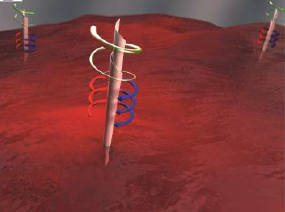
\includegraphics[width=0.5\textwidth]{nanoJet3}
  \caption{Demonstrating the drilling motion of the nanotubes under rotating
 magnetic field~\citep{C2NR32798H}.}
  \label{nanotube}
\end{center}
\end{wrapfigure}
%\end{figure}

Alternatively, the micro driller can be powered and controlled by using an external magnetic field 
such that changes in the frequency of the rotating magnetic field switch the rotational orientation of the 
micro tool from the horizontal position to the vertical one. The vertical orientation of the rolled up microtube 
and its sharp helical design makes the device suitable for drilling into biological tissue. In addition, the micro 
driller can be used for targeted drug delivery in MIS ~\citep{C2NR32798H}. 


\subsection{Plant-based microrobots}
%\hilight{details about fabrication, extract xylem tissue}
The helical microstructures are not limited to having flagellum-like structures and microbots with
general cilia-like feature have been designed. \citeauthor{gao2013bioinspired}
 observed the helical microstructures that imitates spiral water-conducting vessels of different plants. 

\begin{figure}
  \centering
    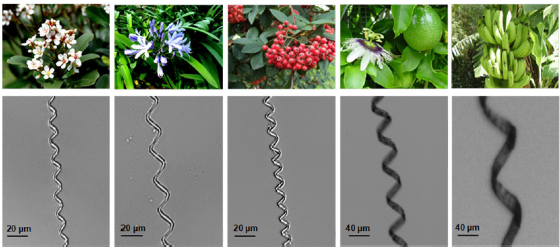
\includegraphics[width=0.9\textwidth]{plants}
  \caption{The shape of the Xylem in differnt plants .~\citep{mahoney2011velocity}.}
  \label{plants}
\end{figure}

In order to obtain unstretched spiral vessel several plants were collected and their leaves were 
macerated and washed with pure water. Tweezers were used to uncover compressed spiral vessels 
in the planar networks. Leaves were gently scored and two segments were pulled apart to a permanent
 length to stretch the spiral vessels. These spiral vessel were kept in a glass slides and covered with a 
thin layer ($20 nm$) of titanium and nickel ($80 nm$) using an 
E-beam evaporator ~\citep{mahoney2011velocity}. The helical vessels were coated in nail 
polish and baked for 2 minutes to impound the helix and protect the structure. The final product is 
a photoresist film on glass that was cut into required lengths.      
  

The fabrication process involves coating isolated spiral xylem vessel plant fibres within a (Figure~\ref{ref8})
thin magnetic layer. Xylem tissue transports the plant\rq{}s required food such as water and other 
nutrition from the root to the leaves using capillary action ~\citep{mahoney2011velocity}.
Use of plant material in this method enables simple three-dimensional microswimmers fabrication 
and biocompatibility. In addition, the magnetic cover helps to ensure accurate directional control and 
high-speed propulsion. Therefore the fabrication processes were extremely simplified as the main 
component of the helical microswimmers is from nature and more than a million individual micro helicals 
can be made from a very small section of the plant stalk ~\citep{mahoney2011velocity}. 


Using mechanical stretching can control geometric variables of the helical vessels such as the pitch and
 helix angle and hence plenty of helical microswimmers can be reproduced. The final shape of the 
helical microswimmer is determined mainly by the initial diameter of the unstretched spiral vessel. The
 process of stretching helical plant structure was performed via plastic deformation so that the number 
of helical turns are constant and tensile stretching of the plant fibre stretching is negligible~\citep{mahoney2011velocity}. 


%\begin{figure}
%  \centering
\begin{wrapfigure}{r}{0.5\textwidth}
  \begin{center}
    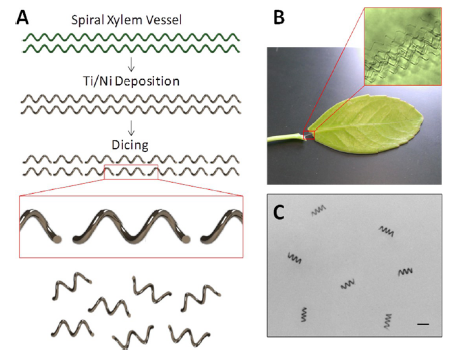
\includegraphics[width=0.5\textwidth]{plants2}
  \caption{(A) The stages were required to make a plant-based microrobot. (B) A microscopic image of the 
a xylem helical structure. ~\citep{gao2013bioinspired}.}
  \label{plants2}
\end{center}
\end{wrapfigure}
%\end{figure}


The method used for precise propulsion control and characterising the locomotion behaviour of the 
plant-based microswimmers is similar to the method applied in \citeauthor{gao2013bioinspired} study.

According to \citeauthor{gao2013bioinspired} ~\citep{gao2013bioinspired} experiment, the plant-based 
microswimmers exhibited high speed movement ($85~\mu m$) in raw biological medium such as 
pure human serum under the rotating magnetic field. However, their swimming speed in pure water
 ($90~\mu m$) was slightly higher than human serum.   
 Hence, an increased velocity of the 
biological fluid has a minor effect on the plant-driven microswimmers, which is an important 
advantage of this microdevice over the common microrobots%\hilight{WHY}.




\subsection{Jellyfish style microrobots}
For the purpose of this project different proposed structures of microrobots were studied
 and analysed. This will enable helical microswimmers to be reproduced. Once reproduced, the aim of this project will be to compare
 the efficiency, power, motion velocity and cost-efficiency of various microrobot designs for mass production
 of the microswimmers. The fabrication of microswimmers will be by Nanoscribe facility using 3D laser
 lithography. After the microrobots are produced their characteristic will be analysed
 under the scanning electron microscope in order to identify further improvements in microrobot design. 



\section{Fabrication methods} \label{fabrication}

Historically, the fabrication of the microrobot was the main problem that recent fabrication methods 
offer a feasible solution~\citep{gao2013bioinspired}.
In 2007, the first artificial bacteria flagella was fabricated based on thin-film deposition and self-scrolling
 methods~\citep{qiu2014noncytotoxic}.\hilight{In this method}. They used InGaAs/GaAs bilayer for fabricating
helical tail and Ni for actuation microrobot\rq{}s head. The similar fabrication method employed by Zhang
 in 2009 with the addition of a Cr layer between the microrobots\rq{} tail and its head~\citep{qiu2014noncytotoxic}.
An improved adhesion of microrobot was the result of adding Cr layer. 

3D laser direct writing (DLW) and electron beam decomposition are methods used since then. A typical 
fabrication process consists of two stages. Initially the core structure of the artificial helical 
microswimmer is printed using 3D lithography and then electron beam evaporation is used for 
ferromagnetic thin film coating~\citep{tottori2013artificial}.  
Performance of each microswimmer (with different design) can be imaged by the scanning electron
 microscope (SEM). After the fabrication process is completed, the next step is to release the structure into 
deionised water using the tungsten probe. The tank with deionised water is installed in the middle of the 
three-axis Helmholtz setup. 



To improve biocompatibility for in-vivo applications, the 
microrobot can be covered with a thin layer of titanium. In addition, the microrobot\rq{}s structure was layered with 
nickel for the purpose of magnetic actuation.

\citeauthor{qiu2014artificial}~\citep{qiu2014artificial} reported a successful application of helical microrobots
for drug delivery were known as \lq\lq{}smart\rq\rq{} drug carriers. They used DLW for the fabrication method which 
was consisted of three steps as shown in the Figure \ref{tempreture}. 



The smart drug carriers were coated in a layer of temperature-sensitive liposomes which is composed 
of a lipid bilayer and was proposed for cancer therapy in local hyperthermia treatments~\citep{qiu2014artificial}.
The main component of temperature-sensitive liposomes is Dipalmi- toylphosphatidylcholine (DPPC) which
transforms from solid to liquid gel at the $41^{\circ} C$ and released encapsulated drugs.

\paragraph{}
 \citeauthor{qiu2014noncytotoxic}~\citep{qiu2014noncytotoxic} were used commercially available material such as ORMOCOMP
 for fabrication of helical microrobots in their recent experiment. ORMOCOMP is a biocompatible photoresist which
can improve the potential use of microrobots for in vivo applications becuase it supports viability, cell proliferation
 and normal morphology of various cell lines. For the purpose of magnetic microrobot actuation, soft magnetic material
such as Fe, Ni and Co are commonly used in microscale structures. The main reason is their biocompatibility
with surface decomposition methods, however Ni and Co are cytotoxic and pure iron can be biodegradable~\citep{qiu2014noncytotoxic}.
ORMOCOMP helical swimmers were coated onto a thin layer of Fe ($25 nm$) using electron beam decomposition.
  

%\begin{figure}
%  \centering
\begin{wrapfigure}{r}{0.5\textwidth}
  \begin{center}
    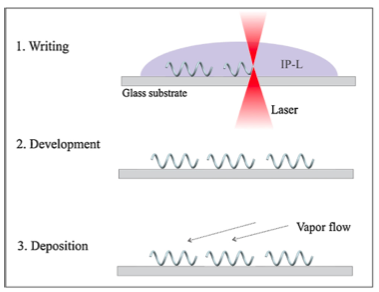
\includegraphics[width=0.5\textwidth]{tempreture}
  \caption{DLW steps. step 1 is writting helical microrobots, in step 2 microrobots were 
developed in isopropyl alcohol and step 3 is coating them by a layer of Ni and Ti. ~\citep{qiu2014artificial}.}
  \label{tempreture}
\end{center}
\end{wrapfigure}
%\end{figure}





%%%%%%%%%%%%%%% Table %%%%%%%%%%%%%%
\begin{table}[h!]
  \centering

\setlength{\arrayrulewidth}{.6mm}
\setlength{\tabcolsep}{1pt}
\renewcommand{\arraystretch}{2.8}


  \begin{tabular}{ c m{2.5cm}  m{4.3cm} m{3cm} m{2cm}}
    \hline
\rowcolor{lightgray}
    Microrobot Image & Design  & Fabrication Method & propulsion method	&Citation  \\ \hline\hline



    \begin{minipage}{.3\textwidth}
      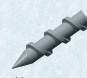
\includegraphics[width=\linewidth, height=25mm]{screw_ta}
    \end{minipage} 
    &
    \begin{minipage}[t]{3cm}
      \begin{itemize}
        \item Helical Screw Shape
    
      \end{itemize}
    \end{minipage}
    & 
    \begin{minipage}{4cm}
      \begin{itemize}
        \item Direct Laser Writting (DLW)
	\item Two-photon Polymerization
   
      \end{itemize}
    \end{minipage}
	&

	&
	   \begin{itemize}
        \item \citep{peyer2013magnetic}
   
      \end{itemize}
    \\ \hline
%%%%%%%%%% Second Row

 \begin{minipage}{.3\textwidth}
      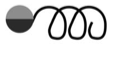
\includegraphics[width=\linewidth, height=25mm]{helical_rigid_tail}
    \end{minipage}
    &
    \begin{minipage}[t]{3cm}
      \begin{itemize}
        \item Helical rigid tail
      
      \end{itemize}
    \end{minipage}
    & 
    \begin{minipage}[t]{4cm}
      \begin{itemize}

        \item Direct Laser Writting (DLW)
	\item Two-photon Polymerization
   
      \end{itemize}
    \end{minipage}

	&


	&
	   \begin{itemize}
        \item \citep{peyer2013bio}
   
      \end{itemize}
    \\ \hline

%%%%%%%%%%%%%%%% Third row

\begin{minipage}{.3\textwidth}
      \includegraphics[width=\linewidth, height=25mm]{Planar_flexible_tail}
    \end{minipage}
    &
    \begin{minipage}[t]{3cm}
      \begin{itemize}
        \item Planar flexible tail
     
      \end{itemize}
    \end{minipage}
    & 
    \begin{minipage}[t]{4cm}
      \begin{itemize}
        \item The EMA coil system
     
      \end{itemize}
    \end{minipage}
&


	&
	   \begin{itemize}
        \item \citep{ko2012jellyfish}
   
      \end{itemize}
    \\ \hline

%%%%%%%%%%%%% Forth row

\begin{minipage}{.3\textwidth}
      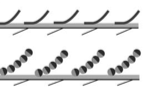
\includegraphics[width=\linewidth, height=25mm]{cilia-shape}
    \end{minipage}
    &
    \begin{minipage}[t]{3cm}
      \begin{itemize}
        \item Cilia
     
      \end{itemize}
    \end{minipage}
    & 
    \begin{minipage}[t]{4cm}
      \begin{itemize}
        \item The EMA coil system
     
      \end{itemize}
    \end{minipage}
&


&
	   \begin{itemize}
        \item \citep{ko2012jellyfish}
   
      \end{itemize}
    \\ \hline



%%%%%%%%% Fifth Row
 \begin{minipage}{.3\textwidth}
      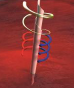
\includegraphics[width=\linewidth, height=25mm]{tube_ta}
    \end{minipage}
    &
    \begin{minipage}[t]{3cm}
      \begin{itemize}
        \item Nanotube
        
      \end{itemize}
    \end{minipage}
    & 
    \begin{minipage}{4cm}
      \begin{itemize}
        \item Molecular Beam Epitaxy (MBE)
	   
	   
    
      \end{itemize}
    \end{minipage}
	&




	&
	   \begin{itemize}
        \item \citep{C2NR32798H}
   
      \end{itemize}
    \\ \hline

%%%%% Sixth Row

 \begin{minipage}{.3\textwidth}
      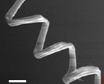
\includegraphics[width=\linewidth, height=25mm]{plant_ta}
    \end{minipage}
    &
    \begin{minipage}[t]{3cm}
      \begin{itemize}
        \item Plant-based
      
      \end{itemize}
    \end{minipage}
    & 
    \begin{minipage}[t]{4cm}
      \begin{itemize}
        \item Macerating Plant\rq{}s Leaves
	\item Seperating Spiral Vessels
	\item Stretching spiral Vessels
	\item Coating with Ti

      \end{itemize}
    \end{minipage}
	&



	&
	   \begin{itemize}
        \item \citep{gao2013bioinspired}
   
      \end{itemize}
    \\ \hline

%%%%%% Seven Row

 \begin{minipage}{.3\textwidth}
      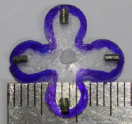
\includegraphics[width=\linewidth, height=25mm]{Jelly}
    \end{minipage}
    &
    \begin{minipage}[t]{3cm}
      \begin{itemize}
        \item Jellyfish
     
      \end{itemize}
    \end{minipage}
    & 
    \begin{minipage}[t]{4cm}
      \begin{itemize}
        \item The EMA coil system
     
      \end{itemize}
    \end{minipage}
&



	&
	   \begin{itemize}
        \item \citep{ko2012jellyfish}
   
      \end{itemize}
    \\ \hline








  \end{tabular}
  \caption{Different types of microrobots and their fabrication method.}\label{Micro}
\end{table}


%%%%%%%%%
%%%%%%%%%%%%%%%%%%%% Method %%%%%%%%%%%%%
%%%%%%%%%

\chapter{Methods}

%%%%%%%%%%%%%%%%%% Structure %%%%%%%%%%%%%
\section{Microrobot structure}

One of the main requirement of the magnetic microrobot is using magnetic material in their structure 
to perform actuation task~\citep{qiu2014noncytotoxic}. 







%%%%%%%%%%%%%%%%%%% Design %%%%%%%%%%%%%%%
\section{Microrobot design}

%The lenght of the microrobots used by \citeauthor{qiu2014noncytotoxic}~\citep{qiu2014noncytotoxic} was
%15.7 \mu m$ and its diameter was $5.3 \mu m$. 


%--------------- Table of all design of the microrobots------------------------















\begin{table}[!ht]

\centering% used for centering table
{\rowcolors{2}{gray!100!brown!70}{gray!50!yellow!30}
\begin{tabular}{c c c c c c c c}% centered columns (8 columns)
\toprule[2.0pt]



\head{Author} & \head{Shape} & \head{Length} & \head{Pitch} & \head{Pitch-angle} & \head{Radius} & \head{Filament-radius} & \head{Speed}\\

%heading
\midrule
%\hline% inserts single horizontal line
Arcene 	& 	    		  & 	1000		& 	1000		& 	1000		& 	1000		& 	1000		& 	1000\\% inserting body of the table
Dexter 	& 	Sparse 		  & 	20000	& 	1000		& 	1000		& 	1000		& 	1000		& 	1000\\
Dorothea & 	Sparse 		  & 	10000	& 	1000		& 	1000		& 	1000		& 	1000		& 	1000\\[1ex]% [1ex] adds vertical space



\bottomrule[2.0pt]
\end{tabular}
}
\label{table:nonlin}% is used to refer this table in the text
\caption{Microrobot\rq{}s design comparisons}\label{design}% title of Table
\end{table}




%-------------------------------------------------------------------------------------------






%%%%%%%%%%%%%%%%%% Fabrication %%%%%%%%%%%%%
\section{Microrobot fabrication} \label{microFabric}
\subsection{}

%--------------- Table of all fabrication of the microrobots------------------------





%%%%%%%%%
%%%%%%%%%%%%%%%%%%%% Testing %%%%%%%%%%%%%
%%%%%%%%%
\chapter{Simulation}

Analysing fluid dynamic phenomena on microorganism is a fundamental approach to model microorganism
 locomotion~\citep{smith2009boundary}.


%\begin{figure}
%  \centering
\begin{wrapfigure}{r}{0.5\textwidth}
  \begin{center}
    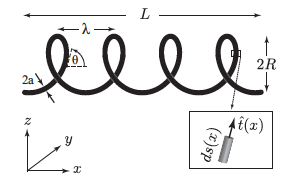
\includegraphics[width=0.5\textwidth]{parameters}
  \caption{The essential helix parameters to design a helical microrobot~\citep{rodenborn2013propulsion}.}
  \label{parameters}
\end{center}
\end{wrapfigure}
%\end{figure}

A helical bacterial flagellum can be uesed as a reference to model a helical microrobot. The 
essential parameters to model a helix are, helix length ($L$), pitch ($\lambda$), pitch angle ($\theta$), 
radius ($R$), filament radius ($a$) and contour length ($\Lambda = L/ \cos \theta$). Figure~\ref{parameters} shows
the helix parameters evidently~\citep{rodenborn2013propulsion}. The flagella parameters were measured for
 several species of bacteria and its result showed the helical pitch is typically ranging between $2R$ and
$11R$, ($2R < \lambda < 11R$). Also the helix length ($L$) varies from $3\lambda$ to $11\lambda$, 
($3\lambda < L < 11\lambda$).


\section{Mathematical model}\label{maths}
The flagella rotation at low Reynolds number exerts an axial thrust ($F$) and torque ($T$) related to the
rotation rate ($\omega$) and flagellum axial velocity ($\nu$). At the same time, fluids was exerted the force
 ($-F$) and the torque ($-T$) on the swimming microrobots~\citep{purcell1997efficiency}. The fluid dynamic 
govern by the Stokes equations (\ref{stokes}) in the low Reynolds regime;


\begin{equation}
  -\nabla{p}+ \eta\nabla^2{\nu}  = 0
\label{stokes}
\end{equation}

Where $\eta$ and $p$ are fluid dynamic velocity and pressure respectively. Therefore thrust ($F$) and 
torque ($T$) are linearly related to the $\nu$ and $\omega$ as there are no derivation of time in 
the equations \ref{stokes}. Thses linear relationship can be defined as follow;


\begin{equation}
  F  = A\nu + B\omega
\label{linear1}
\end{equation}

\begin{equation}
  T = C\nu + D\omega
\label{linear2}
\end{equation}


 Therfore, a matrix 
$\bigl(\begin{smallmatrix}
A&B\\ C&D
\end{smallmatrix} \bigr)$
 defined as propulsion matrix the
model to explain the flagellar swimming motion described by following equation~\citep{rodenborn2013propulsion}
as mentioned in the literature review earlier;
 

\[
\begin{bmatrix} F\\ 
T\end{bmatrix}  = \begin{bmatrix} A & B \\ 
C & D \end{bmatrix}  \begin{bmatrix} \nu
 \\ \omega
\end{bmatrix}
\]

The elements in the symetric $2\times2$ matrix (propulsive matrix) in the above equation only depends on 
flagellum geometry. The propulsive matrix elements can be computed by three methods called;
resistive force theory, slender body theory and regularized Stokeslet theory in sections \ref{method3}, 
\ref{method1} and \ref{method2} respectively. 





\subsection{Resistive force theory}\label{method3}


%\begin{figure}
%  \centering
\begin{wrapfigure}{r}{0.5\textwidth}
  \begin{center}
    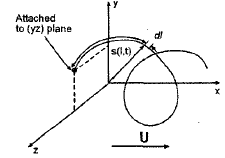
\includegraphics[width=0.5\textwidth]{filament}
  \caption{A motion of an arbitary filament~\citep{edd2003biomimetic}.}
  \label{filament}
\end{center}
\end{wrapfigure}
%\end{figure}


%\begin{figure}
%  \centering
\begin{wrapfigure}{r}{0.5\textwidth}
  \begin{center}
    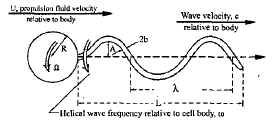
\includegraphics[width=0.5\textwidth]{motion}
  \caption{~\citep{edd2003biomimetic}.}
  \label{motion}
\end{center}
\end{wrapfigure}
%\end{figure}



The swimming velocity and efficiency of the microrobot can be predicted by Resistive force theory (RFT)~\citep{purcell1997efficiency}. 
The force exerted on the fluid by micro swimmer were calculated initially and the micro swimmer will have a net 
movement if the force is not zero~\citep{Doe:2013:Online}. Furthermore, the swimming velocity will decrease if the helical
body attached to the innert head. Figure \ref{filament} shows an arbitary filament motion which is defined by $s(l,t)$. 
A direction of the helix velocity ($U$) is along x-axis and its rotation is symetric about the x-axis. 
The following assumption has been made in order to use the RFT. The geometry
of the helix is on the yz-plane and it always attached to the robot body (can be a sphere). The 
filament motion is periodic and filament length is constant at all the time. Acceleration can be neglected as the
system is in the low Re number fluid. Hence, the equations \ref{thrust} and \ref{torque} will describe the force balance and 
the moment balance in the x-axis direction. The thrust and torque will be determined by integrating over the 
first term of the force balance and moment balance equations (\ref{thrust} and \ref{torque}) 
 respectively ~\citep{edd2003biomimetic}.



\begin{equation}
  \cfrac {1} {\Delta T} \int_0^{\Delta T} \int_0^L  f_x(l,t)\: \mathrm{d}l \:\mathrm{d}t + C_DU  = 0
\label{thrust}
\end{equation}

\begin{equation}
  \cfrac {1} {\Delta T}  \int_0^{\Delta T} \int_0^L [\bold r \bold \times \bold f(l,t)] . \bold e_x \: \mathrm{d}l \:\mathrm{d}t + C_{D\Omega}\Omega= 0
\label{torque}
\end{equation}

Where $\Delta T$ is the time filament motion repeats and integration is taken over the whole lenght $(L)$ of the
helix. 

\paragraph{}
In order to solve the integration problem, the force ($f$) is required to be defined. Therefore, a new
coordination system was introduced and the force vector was defined as a composition of force per unit length
in the normal and tangent directions. Two identical motions are considered for the swmming microrobots
are; rotating and translating (assumed in the x-axis direction). Hence, the force balance and moment balance 
equations are simplified as following; 


\begin{equation}
Nf_xL  + C_DU  = 0
\label{simple_thrust}
\end{equation}



\begin{equation}
 Nf_yAL + C_{D\Omega}\Omega= 0
\label{simple_torque}
\end{equation}

Where $N$ and $A$ are number of filaments and helical amplitude of filaments respectively. Also $f_x$ and 
$f_y$ shows the components of the force vector along x and y directions. In addition, $C_D$ and $C_{D\Omega}$
were computed by equations \ref{Coeff1} and \ref{Coeff2} where $R$ is redius of the helix and $\mu$ is fluid velocity.


\begin{equation}
 C_D  = 6 \pi \mu R
\label{Coeff1}
\end{equation}



\begin{equation}
 C_{D\Omega}= 8 \pi \mu R^3
\label{Coeff2}
\end{equation}

The $f_x$ and $f_y$ are written as composite of forces in the normal and tangent directions;

\begin{equation}
 f_x  = f_t\cos \theta - f_n\sin \theta
\label{normal}
\end{equation}



\begin{equation}
 f_y = f_t\sin \theta + f_n\cos \theta
\label{tangant}
\end{equation}

\begin{equation}
 \tan \theta  = \cfrac{\lambda}{2\pi A}
\label{tang}
\end{equation}



\begin{equation}
 f_t = -C_t(U \cos \theta - \omega A \sin \theta)
\label{normal_f}
\end{equation}



\begin{equation}
f_n = - C_n(-U \sin \theta - \omega A \cos \theta)
\label{tangant_f}
\end{equation}

Where $C_t$ and $C_n$ called resistance coefficients ~\citep{edd2003biomimetic};
 

\begin{equation}
 C_t = \cfrac{2 \pi \mu}{\ln (\cfrac{2 \lambda}{b}) - \cfrac{1}{2}}
\label{Coeffient1}
\end{equation}



\begin{equation}
 C_n = \cfrac{4 \pi \mu}{\ln (\cfrac{2 \lambda}{b}) + \cfrac{1}{2}}
\label{Coeffient1}
\end{equation}

Microrobot\rq{}s swimming speed and rotation rate weer determined by solving 
the equations \ref{normal_f} and \ref{tangant_f}. Therefore, thrust ($F$), torque ($T$) and drag ($D$) 
on flagellum can be predict by following equations~\citep{rodenborn2013propulsion};

\begin{equation}
 F = (\Omega R)(C_n - C_t) \sin \theta \cos \theta \cfrac{L}{\cos \theta} 
\label{thrust}
\end{equation}

\begin{equation}
 T = (\Omega R^2)(C_n \cos ^2 \theta + C_t \sin ^2 \theta) \cfrac{L}{\cos \theta}
\label{torque}
\end{equation}

\begin{equation}
 D = U (C_n \sin ^2 \theta + C_t \cos ^2 \theta) \cfrac{L}{\cos \theta} 
\label{drag}
\end{equation}



Finally, the efficiency of the helical swimmers can be computed as follow;



\begin{equation}
 efficiency = \cfrac{FU}{T \omega} 
\label{efficiency}
\end{equation}

 

\citeauthor{rodenborn2013propulsion}~\citep{rodenborn2013propulsion} demonestrated the failure of resistive force
 theory to predict thrust and drag in microrobots motion accurately. The reason of the failure was neglecting hydrodynamic
interaction between flows induced by different parts of a flagellum. In particular, helical flagellum with
 smaller pitch ($\lambda$) will have smaller separation of filament segments (Figure~\ref{parameters}). Hence,
 the hydrodynamic interaction between different parts of a flagellum becomes stronger and in very small
pitch ($\lambda \to 0$) the helix converts to a cylinder which has no thrust ($F= 0$).

 





\subsection{Regularized Stokeslet method}\label{method2}

A regularization parameter can be used as a proxy for the body radius to minimise numerical errors
 in modelling a flagellum as a one dimentional filament in a low Reynolds~\citep{smith2009boundary}.
number fluids. The Regularized Stokeslet method (RSM) is one of the approch to solve the zero 
Reynolds number linear \lq{}Stokes flow\rq{} equations;



\begin{equation}
 \left.\begin{aligned}
        0 &= - \nabla p + \mu \nabla ^ 2 u + f \\
        0 &=\nabla . u
       \end{aligned}
 \right\}
 \qquad \text{Stokes flow equations}
\label{stokes}
\end{equation}

where $u$ (velocity), $p$ (pressure), $\mu $ (kinematic viscosity), and $f$ (force) are measured per unit
volume. The singular \lq{}Stokeslet\rq{} solution for the equations \ref{stokes} corresponds to the purely 
viscous component (point force) of the flow which was determined by moving sphere. 
The \lq{}Stokeslet\rq{} solution for unit force acts in the j-direction and concentrated at $\xi $, where $f$ is;
  

\begin{equation}
 f (x) = \delta (x - \xi) e_j 
\label{force}
\end{equation}

$\delta (x - \xi)$ is called Dirac delta distribution. The velocity in the i-direction driven by this force is defined
 as follow;


\begin{equation}
 S _{ij} \bm{(x , \xi)} = (\frac{\delta _{ij}}{r} + \frac{r_i r_j}{r^3})
\label{i-direction}
\end{equation}

Where $\delta _{ij}$ denotes Kronecker delta tensor, $r_i = x_i - \xi _i$ and $r^2 =| \bm{x}- \bm{\xi} |^2 = r_1 ^2 + r_2 ^ 2 + r_3 ^2$.
The flow concentrates at point $\bm \xi$ by the force $\bold F$ where $ \bm{f (x)} = \delta (\bm{x} - \bm{\xi) F}$.
The solution is given by finding the velocity $u_i(\bm x)$;

\begin{equation}
 u_i(x) =(\frac{1}{8 \pi \mu}) S_{ij}\bm{( x, \xi)} F_j
\label{velocity}
\end{equation}

The resistive force theory (RFT) and slender body theory (SBT) for modelling of flagellum driven 
flow were formed on the base of the Stokeslet~\citep{smith2009boundary}. These methods solved the 
three dimentinal flow problem with flexible boundaries without using direct computation for the differential
equations. Therefore, the provided solution are extremely efficient in terms of computational costs. The fluid
velocity was modeled by the following equation;
   


\begin{equation}
\bold {u(x)} =(\frac{1}{8 \pi \mu}) \int_S \mathrm \bm{f(\xi)} . \bm{S( x, \xi)}\, \mathrm{d}S_{\xi}
\label{fluid_velocity}
\end{equation}

Where $S$ is a collection of lines or surfaces of flagella, $\bm{f(\xi)}$ shows force per unit length or area.
$\bm{f(\xi)} dS_{\xi}$ denotes the force flagella body exerted on the fluid and $-\bm{f(\xi)} dS_{\xi}$ is the 
force fluid applies to the body. The flagella is represented by equation \ref{fluid_velocity} with the boundary
$S$ and parameter $\bm{\xi (s)}$ where $0 < s <1$ is scaled arclength parameter. However, the flow field
at any point $\bm{x} = \bm{\xi} (s)$ is sigular and the collection of points on the surface of the filament 
are required to calculate the force per unit length. The collection of points were replaced on a small distance 
from the centreline;

\begin{equation}
\bold {X(s_q)} = \bm{\xi}(s_q) + a(s_q) \bm{n}(s_q)
\label{centreline}
\end{equation}

where $a(s_q)$ is a radius of slender body and $\bm{n}(s_q)$ is a unit normal vector. Point distributions of 
Stokeslets at any point $x = \bm{\xi}_q$ and line distribution inside the notional surface
of the flagella are both singular. However, surface distributions of Stokeslets do not result in singular  velocity
 but it still require attentive numerical implementations~\citep{smith2009boundary}. The \lq{regularized Stokeslet}\rq{}
 introduced an exact solution for the equations \ref{stokes_reg} to overcome these issues. 
This method used a cut off function ($\psi$) with a regularization parameter ($\epsilon$) to smooth point forces 
such that $\int_{R^3} \psi_{\epsilon} (\bm{x})\, \mathrm{d}V_x = 1$.



\begin{equation}
 \left.\begin{aligned}
        0 &= - \bm{\nabla} p + \mu \nabla ^ 2 \bm{u} + \bm{f} \psi_\epsilon (\bm{x} - \bm{\xi}), \\
        0 &=\bm{\nabla . u}
       \end{aligned}
 \right\}
 \qquad \text{Stokes flow equations with regularization parameter}
\label{stokes_reg}
\end{equation}

In RSM method, with a assumption of $\psi_{\epsilon}(\bm{x} - \bm{\xi}) := 15\epsilon^4 /8\pi \mu r_{\epsilon}^7$ 
and $r_{\epsilon} = \sqrt{r^2 + \epsilon ^2}$ the regularized Stokeslet velocity tensor measured by the the following:


\begin{equation}
 S _{ij}^{\epsilon} \bm{(x , \xi)} = \frac{\delta _{ij}(r^2 + 2{\epsilon}^2) + r_i r_j}{r_{\epsilon}^3}
\label{velocity-tensor}
\end{equation}

Therefore the boundary for intergal equation (\ref{fluid_velocityReg}) is defined and the fluid velocity at location $x$ is;

\begin{equation}
\bold {u(x)} =(\frac{1}{8 \pi \mu}) \int_S \mathrm \bm{f(\xi)} . \bm{S^{\epsilon}( x, \xi)}\, \mathrm{d}S_{\xi}
\label{fluid_velocityReg}
\end{equation}

Where 


























\subsection{Slender body theory}\label{method1}



%%%%%%%%%
%%%%%%%%%%%%%%%%%%%% Testing %%%%%%%%%%%%%
%%%%%%%%%
\chapter{Experiments}

% Table show the range of wireless microrobopts input frequency and their speed.

Fe-ABF and FeTi-ABFs 
two magnetic fields of strenghts 1mT and 3 mT
The test show that forward speed is increasing with increasing input frequency below a critical value
 called (step-out frequency is the maximum magnetic field frequency that the ABFs can follow synchronously).
The step out frequency increases with the strength of the magnetic field. the maximum speed of Fe-ABF was
48.9 $\mu ms^{-1}$ at the field strength of $9 mT$ and $72 Hz$ ~\citep{qiu2014noncytotoxic}.


%%%%%%%%%
%%%%%%%%%%%%%%%%%%%% Results %%%%%%%%%%%%%
%%%%%%%%%
\chapter{Results}



%%%%%%%%%
%%%%%%%%%%%%%%%%%%%% Discussion %%%%%%%%%%%%%
%%%%%%%%%
\chapter{Discussion}




%%%%%%%%%
%%%%%%%%%%%%%%%%%%%% Conclusion %%%%%%%%%%%%%
%%%%%%%%%
\chapter{Conclusion and future work}






\renewcommand{\bibname}{References}
\bibliographystyle{plainnat}
\bibliography{References} 
%\addcontentsline{toc}{chapter}{\numberline{}References}

\end{document}